\documentclass[a4paper,12pt]{article}

\usepackage{amsfonts}
\usepackage[T1]{fontenc}
\usepackage[utf8]{inputenc}
\usepackage{amsmath}
\usepackage{graphicx}

\title{Progettazione del database}

\begin{document}
\maketitle

In questo documento verranno descritte le specifiche e la struttura del database relativo al lato server. Il modello di sviluppo che si vuole seguire è quello di un database relazionale quindi nella prima sezione verranno mostrate le specifiche, in seguito lo schema entity-relationship e in fine lo schema logico che verrà implementato sul DBMS. 

\section*{Specifiche}
Il database deve contenere i dati relativi agli utenti registrati. Le credenziali da tenere in memoria per ogni utente sono l'email, la password di accesso, l'ultima posizione rilevata e se è attivo oppure no. Per ogni utente viene creato un personaggio(sviluppo futuro: per ogni utente più personaggi) del quale si conosce la classe e le statistiche attuali di gioco, Vita, Attacco e Difesa. La classe determina le statistiche iniziali di gioco, gli attacchi del personaggio e il modo in cui si sviluppa. 
\section*{Schema Entity-Relatioship}
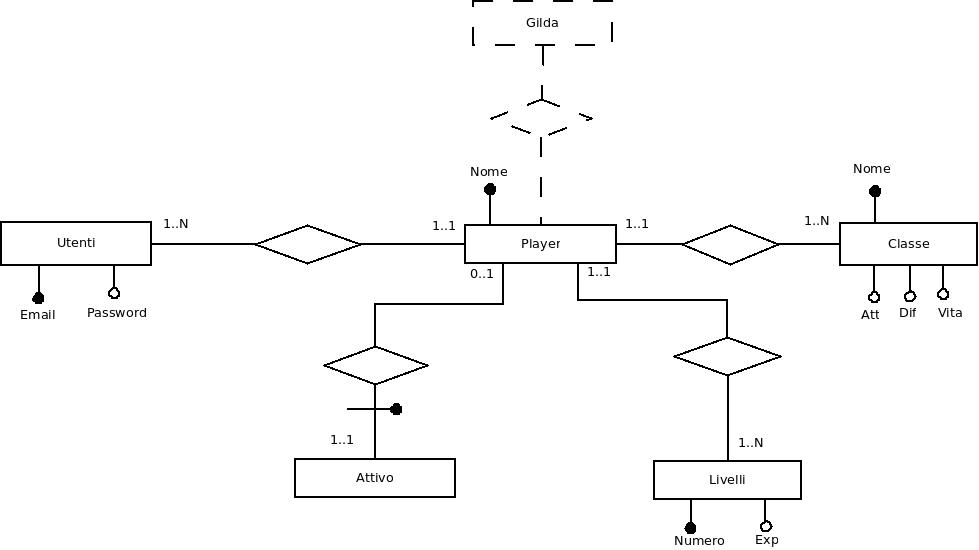
\includegraphics[scale=0.4]{SchemaER.jpeg}

\end{document}